%\title{Ising Convolutional RBM}
%\author{Emanuel Casiano-Diaz}
%\date{May 18, 2022.}


%Formatting Packages
\documentclass[12pt, two sided]{article}
\usepackage[utf8]{inputenc}
%\usepackage[letter,top=1.1in,bottom=1.1in,left=1.6in,right=1.1in]{geometry}
\usepackage[letterpaper,margin=1in]{geometry}

\usepackage{graphicx}
\usepackage{subfig}
\usepackage{float}

%Math Packages
\usepackage{amsmath}
\usepackage{amssymb}
\usepackage{bm}
\DeclareMathOperator{\Tr}{Tr}

%Physics Package
\usepackage{physics}

%Allow accentuation marks
\usepackage[utf8]{inputenc}
\usepackage[T1]{fontenc}

%Image packages
\usepackage{graphicx}
\graphicspath{ {Images/} }

%Enumerating lists
\usepackage{enumerate}% http://ctan.org/pkg/enumerate

%Adjust depth of subsections
\setcounter{secnumdepth}{3}

%Adjust depth of table of contents
\setcounter{tocdepth}{3}

%References Packages
%\usepackage{biblatex}
%\addbibresource{references.bib}
\usepackage[bookmarks=true]{hyperref}
\hypersetup{
    hidelinks=true,
    linkcolor=blue,
    filecolor=magenta,      
    urlcolor=cyan,
}

%Commands and packages imported from particle entanglement paper
\usepackage{amsmath}
\usepackage{xcolor}
\usepackage{graphicx}
\usepackage{amssymb}

\newcommand{\eket}[1]{\bigl \vert #1 \bigr \rangle}
\newcommand{\R}{\boldsymbol{R}}
\newcommand{\Rt}{\tilde{\R}}
\newcommand{\ebra}[1]{\bigl \langle #1 \bigr \vert}
\newcommand{\eexp}[1]{\bigl \langle #1 \bigr \rangle}
\newcommand{\figref}[1]{Fig.~\ref{#1}}
\renewcommand{\vec}[1]{\boldsymbol{#1}}
\newcommand{\ren}{R\'{e}nyi~}
\newcommand{\rnote}[1]{{\it \textcolor{red}{#1} }}
\newcommand{\Eqref}[1]{Eq.~\eqref{#1}}

%Copied from paper
\usepackage{color}
\usepackage{graphicx}
\usepackage[color=green!60]{todonotes}
\usepackage{physics}
\usepackage{amsthm}
\usepackage{amsmath}
\usepackage{amssymb}
\usepackage{enumerate}
\usepackage{placeins}
\usepackage{booktabs}
\usepackage{dsfont}

%For reference formatting
\usepackage[numbers,sort&compress]{natbib}
\bibliographystyle{nsf_new_url}

\setlength{\footskip}{22pt}

 %Line spacing
\usepackage{setspace}
\doublespace

% --------- Begin Document -------- %
\begin{document}

%----- Introduction -------%


\section{Introduction}

%-----------------------------   Symmetry Implementation ----------------------------------------------% 

\section{Symmetry implementation}

To perform the rotational symmetrization, the current general strategy is to choose a $3\times3$ convolutional kernel, place the origin at the center element, then find the groups of vectors with respect to this origin that correspond to $90^\circ$ rotations of each other. 

\begin{figure}[h!]
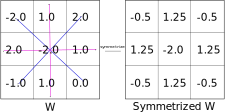
\includegraphics[width=\textwidth]{../figures/symmetrization_diagram.pdf}
\end{figure}

At the moment, we are obtaining inconsistent results. For some runs, the CRBM samples the correct states and observables, but for others it does not. We would like to then take a look at the structures of the kernels if no symmetrizations were applied to the CRBM. In the paper, it is hypothesized that the CRBM should learn the Ising model symmetries, which are: spin flip, mirror, and rotational.

\begin{figure}[h!]
\includegraphics[width=\textwidth]{../figures/T_4.0_kernelDims_2-3_withRotations.pdf}
\caption{Example of a learned kernel at $T=4.0$ by hard-coding rotation symmetry as prescribed.}
\end{figure}

\begin{figure}[h!]
\includegraphics[width=\textwidth]{../figures/L_100_T_4.0_kernelSize_3_crbm_with_rotation_every_step.pdf}
\caption{Example of a learned kernel at $T=4.0$ by hard-coding rotation symmetry as prescribed.}
\end{figure}


%-----------------------------   CRBM without symmetrization ----------------------------------------------% 

\section{CRBM without symmetrization}

In this section, CRBM's with no symmetrization are explored for various hyperparameters. The motivation for this is two-fold: 1) See if the kernels learn Ising Model symmetries and 2) understand what hyperparameters lead to better performance.The training for all networks has been set to stop once the loss function becomes less than $10^{-4}$. Energies sampled from the CRBM will be for an Ising lattice of linear size $L=100$, since the regime where the CRBM beats Metropolis-Hastings is $L\geq100$. The number of samples will be set to $100,000$.

\subsection{Kernel number comparison ($T=4.0$)}

What is the effect of using different number of kernels?

\begin{figure}[h!]
\includegraphics[width=\textwidth]{../figures/T_4.0_kernelDims_1-3_no_symmetries.pdf}
\caption{One $3\times3$ kernel}
\end{figure}

\begin{figure}[h!]
\includegraphics[width=\textwidth]{../figures/L_100_T_4.0_kernelDims_1-3_no_symmetries.pdf}
\caption{Final state and energy of one $3\times3$ kernel}
\end{figure}

\begin{figure}[h!]
\includegraphics[width=\textwidth]{../figures/T_4.0_kernelDims_2-3_no_symmetries.pdf}
\caption{Two $3\times3$ kernels}
\end{figure}

\begin{figure}[h!]
\includegraphics[width=\textwidth]{../figures/L_100_T_4.0_kernelDims_2-3_no_symmetries.pdf}
\caption{Final state and energy of two $3\times3$ kernels}
\end{figure}

\begin{figure}[h!]
\includegraphics[width=\textwidth]{../figures/T_4.0_kernelDims_4-3_no_symmetries.pdf}
\caption{Four $3\times3$ kernels}
\end{figure}

\begin{figure}[h!]
\includegraphics[width=\textwidth]{../figures/L_100_T_4.0_kernelDims_4-3_no_symmetries.pdf}
\caption{Final state and energy of four $3\times3$ kernels}
\end{figure}

\subsection{Kernel size comparison}

What is the effect of varying the linear size of the kernel?

\begin{figure}[h!]
\includegraphics[width=\textwidth]{../figures/T_4.0_kernelDims_2-2_no_symmetries.pdf}
\caption{Two $2\times2$ kernels}
\end{figure}

\begin{figure}[h!]
\includegraphics[width=\textwidth]{../figures/L_100_T_4.0_kernelDims_2-2_no_symmetries.pdf}
\caption{Final state and energy of two $2\times2$ kernel}
\end{figure}

\begin{figure}[h!]
\includegraphics[width=\textwidth]{../figures/T_4.0_kernelDims_2-3_no_symmetries.pdf}
\caption{Two $3\times3$ kernels}
\end{figure}

\begin{figure}[h!]
\includegraphics[width=\textwidth]{../figures/L_100_T_4.0_kernelDims_2-3_no_symmetries.pdf}
\caption{Final state and energy of two $3\times3$ kernel}
\end{figure}

\begin{figure}[h!]
\includegraphics[width=\textwidth]{../figures/T_4.0_kernelDims_2-4_no_symmetries.pdf}
\caption{two $4\times4$ kernels}
\end{figure}

\begin{figure}[h!]
\includegraphics[width=\textwidth]{../figures/L_100_T_4.0_kernelDims_2-4_no_symmetries.pdf}
\caption{Final state and energy of two $4\times4$ kernel}
\end{figure}

Some of the kernels almost seem to look like the symmetrized one, but shifted. What if we do an initial training round, pick the heaviest kernel element, shift it to the center, then symmetrize respect to it?

Another possible source of error is the way that the symmetrization is being implemented. Currently, it is always performed at every training step. In the thesis, they say that the symmetry sampling is performed by randomly picking one of the three symmetries at that step.

% Low temperature


%-----------------------------   ----------------------------------------------% 


%-----------------------------   Energy benchmark ----------------------------------------------% 


%-----------------------------   Wall clock and Autocorrelation times ----------------------------------------------% 




% ------------------------------------------------------ end ---------------------------------- %

% References
\phantomsection 
\addcontentsline{toc}{chapter}{References} 
%\bibliographystyle{apalike} %acm, ieetr, apalike...
 %\section*{Referencess
 \singlespacing
\bibliography{references}

\doublespacing

\end{document}
